\section{Experiments}
\label{sec:experiments}
\subsection{Evaluation metrics}
In order to evaluate the performance of the different algorithms, three different metrics were used. For each of these methods we hold on to the closed world assumption that if a link is not present within the given data set, it should not be a link. 

\subsubsection{Precision and recall} 
Precision and recall can be calculated when the complete system pipeline is used. Precision reflects the fraction of relevant documents from all proposed documents and can thus be calculated as follows:

\begin{align*}
  \textrm{precision} = \frac{|\;\textrm{relevant\;documents} \cap \textrm{retrieved\;documents}\;|}{|\textrm{retrieved\;documents}\;|}
\end{align*}

Within a recommender system, the precision indicates how sensible the proposed links seem to the user. A precision of 50\% means that if for example two links are proposed to the user, at least one of them is correct. If one strives for a high user friendliness of the system, a high precision should be pursued. 

Recall represents the fraction of relevant documents of all originally linked documents and can be calculated as follows:
\begin{align}
  \nonumber \textrm{recall} = \frac{|\;\textrm{relevant\;documents} \cap \textrm{retrieved\;documents}\;|}{|\;\textrm{relevant\;documents}\;|}
\end{align}

The recall thus gives an indication of how well the sytem covers all the documents in the knowledge base. If the main goal of the system is to make the knowledge base as complete as possible, without taking user friendliness into account, a high recall should be obtained. 

The F1-measure can be used to capture both precision and recall into one number. If precision and recall are equally important, this can be calculated in the following way:
\begin{align}
  \nonumber \textrm{F1-measure} = \frac{2*\textrm{recall}*\textrm{precision}}{\textrm{recall} + \textrm{precision}}
\end{align}

All these metrics can be unraveled into precision, recall and F1-measure per
document type to give more insight into the performance of the algorithms with
regards to different document types. 

\subsubsection{K-links}
The k-links metric is used to evaluate the algorithms, without being influenced by the threshold for the number of proposed links. For a document with a given number of correct links, it proposes the same amount of links that the document is known to have. This evaluation metric thus makes the assumption that the algorithm knows in advance how many links should be returned. By doing so, the recall and precision are equivalent since the number of relevant and retrieved document is the same. It prevents the precision from being too optimistic, which would be the case if the fixed number would be lower than the actual amount of links. It also prevents the recall for being too optimistic in the cases that the actual amount of links is lower than the fixed number of proposed links. 

The disadvantage of the k-links metric is of course that it does not take into account the certainty the algorithm has due to the distances. For example, it could be that the distance of the first two ranked documents is very small, but the distance of the third is very large. If the original document has 10 links, the system is forced to additionally return the nine documents, even though these are likely to be wrong because they have a relatively big distance. 

\begin{table}

\begin{tabular}{| l | l | l | l | l | l | l | l |}
\hline
{\bf CORRELATION} & Inf. &  Question &  Good Pr.& Project & Person &  Event & {\bf Average} \\
\hline
Textvectorizer & 20.49 & 42.02 & 30.35 & 25.41 & 5.81 & 21.42 & {\bf 19.73} \\ 
Weighted text & 21.25 & 44.82 & 30.35 & 16.04 & 5.81 & 21.43 & {\bf 19.76} \\ 
Simple tag & 21.33 & 16.67 & 69.64 & 37.81 & 14.87 & 46.83 & {\bf 21.90} \\ 
Tag smoothing & 20.95 & 21.93 & 44.64 & 31.04 & 13.59 & 46.83 & {\bf 20.78} \\ 
Glossaries of tags & 17.70 & 16.67 & 48.21 & 31.46 & 7.95 & 40.47 & {\bf 16.77} \\ 
Weighted tag & 17.70 & 16.67 & 48.21 & 31.46 & 7.95 & 40.48 & {\bf 16.77} \\ 
\hline
\\
\hline
{\bf COSINE} & Inf. &  Question &  Good Pr.& Project & Person &  Event & {\bf Average} \\
\hline
Textvectorizer & 20.49 & 40.70 & 30.36 & 25.42 & 5.81 & 21.43 & {\bf 19.49} \\ 
Weighted text & 21.67 & 44.82 & 30.36 & 16.04 & 5.81 & 21.43 & {\bf 19.90} \\ 
Simple tag & 21.21 & 16.67 & 69.64 & 37.81 & 17.53 & 46.83 & {\bf 22.80 } \\ 
Tag smoothing & 20.58 & 21.93 & 44.64 & 31.04 & 13.59 & 46.83 & {\bf 20.69} \\ 
Glossaries of tags & 18.68 & 16.67 & 48.21 & 31.46 & 10.51 & 40.48 & {\bf 18.02} \\ 
Weighted tags & 18.68 & 16.67 & 48.21 & 31.46 & 10.51 & 40.48 & {\bf 18.02} \\ 
\hline
\\
\hline
{\bf INTERSECTION} & Inf. &  Question &  Good Pr.& Project & Person &  Event & {\bf Average} \\
\hline
Textvectorizer & 4.16 & 3.51 & 10.71 & 19.06 & 0.00 & 24.21 & {\bf 4.45} \\ 
Weighted text & 4.15 & 3.51 & 10.71 & 19.06 & 0.00 & 24.21 & {\bf 4.45} \\ 
Simple tag & 4.15 & 3.51 & 10.71 & 19.06 & 0.000 & 24.21 & {\bf 4.45} \\ 
Tag smoothing & 4.15 & 3.51 & 10.71 & 19.06 & 0.00 & 24.21 & {\bf 4.45} \\ 
Glossaries of tags & 4.16 & 3.51 & 10.71 & 19.06 & 0.00 & 24.21 & {\bf 4.45} \\ 
Weighted tag & 4.15 & 3.51 & 10.71 & 19.06 & 0.00 & 24.21 & {\bf 4.45} \\ 
\hline
\\
\hline
{\bf EUCLIDEAN} & Inf. &  Question &  Good Pr.& Project & Person &  Event & {\bf Average} \\
\hline
Textvectorizer & 3.04 & 3.95 & 17.86 & 0 & 0.85 & 21.43 & {\bf 3.25} \\ 
Tag smoothing & 1.32 & 1.32 & 7.14 & 0 & 0.43 & 0 & {\bf 1.08} \\ 
Simple tag & 14.05 & 10.53  & 30.36 & 38.23 & 14.36 & 35.71 & {\bf 16.56} \\ 
Tag smoothing & 0 & 0 & 0 & 0 & 0 & 0 & {\bf 0} \\ 
Glossaries of tags & 15.64 & 10.53 & 41.07 & 31.46 & 7.95 & 40.47 & {\bf 14.75} \\ 
Weighted tags & 15.64 & 10.53 & 41.07 & 31.46 & 7.95 & 40.47 & {\bf 14.75} \\ 
\hline
\\
\hline
{\bf BHATTACHARYYA} & Inf. &  Question &  Good Pr.& Project & Person &  Event & {\bf Average} \\
\hline
Textvectorizer & 15.57 & 35.88 & 30.36 & 16.15 & 5.30 & 21.43 & {\bf 16.19} \\ 
Weighted text & 18.72 & 29.04 & 30.35 & 11.99 & 7.95 & 21.43 & {\bf 16.63} \\ 
Simple tag & - & - & - & - & - & - & {\bf -} \\ 
Tag smoothing & 4.16 & 3.51 & 10.71 & 19.06 & 0 & 24.2 & {\bf 4.44} \\ 
Glossaries of tags & 18.36 & 17.98 & 48.21 & 48.13 & 10.51 & 40.45 & {\bf 19.39} \\ 
Weighted tag & 18.36 & 17.98 & 48.21 & 48.13 & 10.51 & 40.45 & {\bf 19.39} \\ 
\hline
\end{tabular}

\caption{This table shows the performance based on k-link measuring of all documents. This means that the numbers are the percentage of correctly returned links, given the constraint that the number of links that is returned is equal to the known number of links a document has. These are averages over the entire document base. The left upper corner of each table tells which distance metric was used. Each row describes the performance of one vectorizer. Each column describes the performance of each document type. Thus, the first number 20.49 means that the average percentage correctly returned links of documents of the type 'Information' for the textvectorizer using the correlation distance is 20.49\%.}
\label{klink}
\end{table}

\subsection{Text-based descriptors}
Table \ref{klink} shows the k-link values of all vectorizers, including those of the textvectorizer and the weighted-text vectorizer. The best performance of the textvectorizers is obtained by the cosine distance. This can be attributed
 to the fact that the cosine distance is independent to document length and only
 computes a similarity in document structure. In other words when a document
 has the exact same words as a seconds document but only twice as much the
 cosine similarity classifies these documents as exactly equal. As the textvectorizer
 encodes the number of word occurrences in a vector the cosine distance can 
 easily find document that use the same words frequently.

The cosine distance metric gives the best results for the text vectorizers. On average, 19.49\% and 19.59\% percent of the number of proposed links respectively are correct. The weighted text vectorizer performs a bit better, which is mainly due to an improvement in performance on information and questions.

Both textvectorizers have a low percentage correct with regards to proposing links for Persons. A further analysis shows that 76.36\% (not weighted) and 69.09\% (weighted) of the links for Persons are towards other Persons. However, within the Starfish network such links almost never occur (see table \ref{bayes_table3} for the distribution of document types within Starfish). This could explain the low performance on persons. 

Overall, both textvectorizers are slow in performance even though the corpus is small. Additionally, the the bag-of-words approach imposes a few limitations on the document linker. Firstly, it performs bad when different languages are used. In the case of two different languages, there are less words that the two documents have in common. If important keywords entail word such as `clickers' versus `stemsysteem', there is no way of relating the two documents. Secondly, the current StarFish network consists of mainly textual content. However, in the future this is likely to be extended with images, videos and other non-textual content. These sources should then somehow be converted to text.

Table~\ref{klink} shows the k-link values of all vectorizers, including those
of the textvectorizer and the weighted-text vectorizer. The best performance of
the textvectorizers is obtained by the cosine distance. This can be
attributed to the fact that the cosine distance is independent to document
length and only computes a similarity in document structure. In other words
when a document has the exact same words as a seconds document but only twice
as much the cosine similarity classifies these documents as exactly equal. As
the textvectorizer encodes the number of word occurrences in a vector the
cosine distance can  easily find document that use the same words frequently.

The cosine distance metric gives the best results for the text vectorizers. On
average, 19.49\% and 19.59\% percent of the number of proposed links
respectively are correct. The weighted text vectorizer performs a bit better,
which is mainly due to an improvement in performance on information and
questions. % ROBBERT, FIND SOME QUALTITATIVE EXAMPLES FOR THIS. 

Both textvectorizers have a low percentage correct with regards to proposing
links for Persons. A further analysis shows that 76.36\% (not weighted) and
69.09\% (weighted) of the links for Persons are towards other Persons (see
appendix X). However, within the Starfish network such links almost never occur
(see table~\ref{bayes_table3} for the distribution of document types within
Starfish). This could explain the low performance on persons. 

Overall, both textvectorizers are slow in performance even though the corpus is
small. Additionally, the the bag-of-words approach imposes a few limitations on
the document linker. Firstly, it performs badly when different languages are
used. Figure x shows the differences of vectors of three texts when an English
document is combined with an English proposed document and a Dutch proposed
document. In the case of two different languages, there are less words that the
two documents have in common. If important keywords include words such as
`clickers' versus `stemsysteem', there is no way of relating the two documents.
Secondly, the current StarFish network consists of mainly textual content.
However, in the future this is likely to be extended with images, videos and
other non-textual content. These sources should then somehow be converted to
text.

\subsection{Tag-based descriptors}

\subsubsection{Simple tag similarity vectorizer} 
The performance of the simple tag similarity vectorizer, as shown in
table~\ref{klink} together with the other tag vectorizers, is about 26\%
precision when measuring k-link. The unraveling per document type shows that
Question documents and Person documents perform the worst. This can be
explained by the fact that half of both Questions and Persons have zero tags.
Obviously, the simple tag vectorizer cannot deal with such documents. In fact,
almost all other Questions have only one tag. Since the simple tag vectorizer
compares vectors, it will prefer documents that also have only that particular
tag, which makes it sensitive to attaching Questions to Questions. Something
similar seems to happen with Persons, of which 50.91\% of the connections are
with other Persons.  Apparently, persons with similar expertise are tagged
similarly.  However, as mentioned with the text vectorizer, in Starfish persons
almost never refer to other persons.
Moreover, if a document is badly labeled
this can also induce problems. For example, the question `TurnitIn licence at the 
UvA' has two tags, but the simple tag similarity is unable to find both it's links because 
the link `What is TurnitIn?' is not tagged with `TurnitIn'. The text vectorizer returns both
links correctly. Good practices, events and projects perform better, 
but these document types only make up to 3.2\%, 2.7\% and 5.4\% of the
total amount of documents respectively so have less influence on the average
precision.

\subsubsection{Tag smoothing}
The performance of the simple tag vectorizer, as shown in table~\ref{klink}, is
quite similar with the results of the tag similarity. It performs worse on the
information. This is visible in the `Peer-instruction' information document, in which the tag smoothing fails to make a recommendation the simple tags do. It also
performs worse on Persons, which is visible in the `Claire McDonnell' person document. That document has more tags than average but does not return any correct links.

In the current implementation this vectorizer is relatively slow. In practice
the similarity matrix can be pre calculated and updated in batches. Due to the
transform on the tag similartity matrix, it is very hard to determine which tag
occurrences contributed to the document similarity and why some recommendations
are made. It does not seem to perform much better than the regular bag of words
tag descriptor, in \citeauthor{zhou2011web} the algorithm only starts
performing significantly better when it is presented with more tags.

\subsubsection{Glossaries of tags}
The glossaries of tags approach returns the lowest results without applying the
threshold. This could be a result of the sheer number of tags which have a glossary. For
example, the documents `Is there an English version in Tentamenlade?', `De toetscyclus' 
and `Wat is het verschil tussen Learning Analytics en TTL?' all have the 
tag `ToetsenEnToetsgestuurdLeren' and at most one other tag with a glossary. 
ToetsenEnToetsgestuurdLeren is a tag with a glossary, but that glossary is one sentence 
long. This results in weak vectors which aren't very well distinctive from other documents 
which have little tags or little tags with glossaries. The information needed to link the 
documents does not seem to be present in the current dataset.


\subsubsection{Weighted tag glossaries}
Table~\ref{klink} shows that the weighted tag vectorizer, an extension of the glossaries of tags vectorizer, performs exactly the same as the glossaries of tags vectorizer. It thus seems that applying the weights has no influence on the performance of this vectorizer. The histogram in figure~\ref{weightedtag} shows the number of tags that appear in a certain amount of documents. From this can be derived that there are many tags that almost all the tags appear in 10 documents or less. There are only a few tags that appear in a lot of documents. Thus, the influence of the weighted tag vectorizer is caused by the fact that many tags assign the same or a similar weight to vector, making it approximately the same as the glossaries of tags vectorizer.  

\begin{figure}
\center
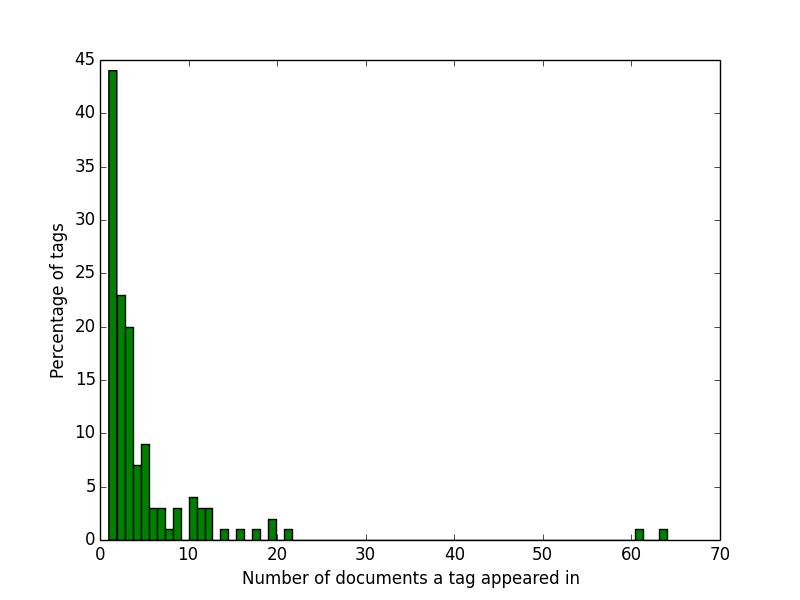
\includegraphics[width =0.6\textwidth]{images/weightedtagexplanation}
\caption{This histogram shows the number of tags that appear in a certain amount of documents. Almost all tags appear in 10 documents or less. Only a few tags are very common and these appear in about 60 different documents.}
\label{weightedtag}
\end{figure}

\subsubsection{Hybrid}
Given the previous results, the best results can be obtained if the textvectorizer and simple tag similarity are combined into one vectorizer. If a document has no tags, it will be handeled by the textvectoriser, otherwise the simple tag similarity will do this. Boht vectorizers use the cosine distance metric. The results are show in table \ref{hybrid}. This hybrid vectorizer performs significantly better than the two vectorizers themselves. 


\begin{table}[h!]
\begin{tabular}{| l | l | l | l | l | l | l | l |}
\hline
 & Inf. &  Question &  Good Pr.& Project & Person &  Event & {\bf Average} \\
\hline
Accuracy hybrid & 21.21 & 31.93 & 69.64 & 37.81 & 19.15 & 46.83 & {\bf 26.13}\\
\hline
\end{tabular}
\caption{This table shows the accuracy of a vectorizer that is a hybrid between the textvectorizer and the simple tag vectorizer using cosine distance. It shows the average percentage of correctly returned links for a given document type if the known number of correct links is proposed by the vectorizer.}
\label{hybrid}
\end{table}

\subsection{Bayesian weighting}
\begin{table}
\begin{tabular}{| l | l | l | l | l | l | l | l |}
\hline
DEVALUATION & Inf. &  Question &  Good Pr.& Project & Person &  Event & {\bf Average} \\
\hline
Textvectorizer & 0.59 & 12.63 & 0.00 & 0.00 & 0.43 & 0.00 & {\bf 2.58}\\
Weighted text vectorizer & 0.59 & 16.58 & 0.00 & 0.00 & 0.43 & 0.00 & {\bf 3.29} \\ 
Simple tag similarity & 1.18 & 10.53 & 0.00 & 4.17& 0 & 0 & {\bf 2.55}\\
Tag smoothing & 0.00 & 10.53 & 0.00 & 4.17 & 0.43 & 0.00 & {\bf 2.33}\\
Glossaries of tags & 4.61 & 13.16 & 0.00 & 6.23 & 6.41 & 0 & {\bf 6.61}\\
Weighted tags & 4.61 & 13.16 & 0.00 & 6.23 & 6.41 & 0 & {\bf 6.61}\\
\hline
\end{tabular}
\caption{The average k-link accuracy per vectorizer per document type if both tag and link devaluation are used to re rank the documents. All vectorizers used the cosine distance.}
\label{bayes_table1}
\end{table}

Table~\ref{bayes_table1} shows the performance of each of the vectorizers (all
with cosine distance) while applying the tag and link devaluation using the
k-link metric. It shows that the performance of all algorithms drastically
decreases when the probabilities are used to re-rank the documents. 
Table~\ref{bayes_table1}  shows the distribution of links in the simple tag
similarity vectorizer, with and without the probabilities (all based on k-link
measuring). It is clear that the links with probabilities have a sharper
distribution: the sparseness of the table shows that many types of links do not
even exist. This effect could be caused by overfitting - the data set could be
too small to calculate reliable probabilities. The preferred effect of having no
Persons link to other Persons was done correctly. However, Good Practices, for
example, are now only assigned to be a person. The vectorizer without
probabilities has a distribution that seems to be more reliable for these types
of documents. The distributions with and without probabilities can be compared
with the original distribution of links in the current Starfish knowledge base,
as shown in table~\ref{bayes_table2}.  

\begin{table}
\begin{tabular}{| l | l | l | l | l | l | l | }
\hline
DEVALUATION & {\bf Inf. }& {\bf Question }& {\bf Good Pr.} & {\bf Project }&{\bf Person }& {\bf Event}  \\
\hline
{\bf Information} & 100.00 &  0.00 &  0.00 &  0.00  & 0.00 & 0.00 \\
{\bf Question} & 11.11 &  84.44  & 0 & 2.22  & 2.22 & 0.00 \\
{\bf Good Practice} & 58.82 &  0.00  &  41.18  &  0.00  & 0.00 & 0.00 \\
{\bf Project }& 93.33 &  3.33  &  0.00  & 0.00 & 3.33 & 0.00 \\
{\bf Person} &  100.00 &  0.00 &  0.00 &  0.00  & 0.00 & 0.00 \\
{\bf Event }& 21.43 &  0.00  &  0.00 &  21.43  & 0.00 & 57.14 \\
\hline
\\
\hline
NO DEVALUATION & {\bf Inf. }& {\bf Question }& {\bf Good Pr.} & {\bf Project }&{\bf Person }& {\bf Event} \\
\hline
{\bf Information} &  21.21 & 16.67 & 69.64 & 37.91 & 17.44 & 46.83 \\
{\bf Question} & 6.67 & 35.56 &17.79 & 4.44 & 35.56 & 0 \\
{\bf Good Practice} & 41.18 & 11.76 & 17.65 & 5.88 & 5.88 & 17.65 \\
{\bf Project } & 30.0 & 16.67 & 6.67 & 13.33 & 20.00 & 13.33 \\
{\bf Person} & 30.01 & 7.27 & 3.64 & 1.81 & 50.01 & 5.45 \\
{\bf Event }& 35.71 & 0.00 & 14.29 & 28.57 & 7.14 & 14.29 \\
\hline
\end{tabular}

\caption{This table shows the percentage of links from one type (row) to another (column) for simple\_tag\_vectorizer with tag and link devaluation (above) and without (below), measured using k-link.  The rows sum up to 100\%. Thus, the first value 100.0\% means that if tag and link devaluation is performed, all proposed links for all newly added documents of the type Information are themselves also Information documents.}
\label{bayes_table2}
\end{table}

\begin{table}
\begin{tabular}{| l | l | l | l | l | l | l | }
\hline
 & {\bf Inf. }& {\bf Question }& {\bf Good Pr.} & {\bf Project }&{\bf Person }& {\bf Event} \\
\hline
{\bf Information} &  39.86 & 8.39 &4.20 &5.59 &37.76 &4.20\\
{\bf Question} & 19.72 &25.35 &12.68 &12.68 &23.94 &5.63\\
{\bf Good Practice} & 25.00 & 17.86 & 7.14 & 10.71 & 25.00 & 14.29 \\
{\bf Project } & 23.91 & 10.87 & 4.35 & 19.57 & 30.43 & 10.87 \\
{\bf Person} & 69.64 & 8.93 & 1.79 & 8.93 & 1.79 & 8.93 \\
{\bf Event }& 28.57 & 0.00 & 14.29 & 9.52 & 33.33 & 14.29\\
\hline
\end{tabular}
\caption{This table shows the percentage of links from one type (row) to another (column) for the links as they are in the document base of Starfish. Thus, the first value 39.86\% means that 39.86\% of the proposed links for Information documents are of the type Question.}
\label{bayes_table3}
\end{table}

Figure \ref{distribution} gives insight into the reason why the probabilities
do not improve the performance. The figure shows a histogram of the percentage
of documents that have a certain probability. The left side shows the
distribution for the tag probabilities, where the red bars represent incorrect
links and the green bars show the correct ones. One would expect that a higher
percentage of correct links would be on the righthand side of the histogram,
since these should have a higher probability. However, this is clearly not the
case. On the contrary, about 75\% of the incorrect links have a chance of
0.0014, the highest probability. The link probability, shown on the right hand
side of the figure, is a bit more promising since the incorrect links are a bit
higher on the left hand side of the histogram. However, there is still no clear
difference in distribution. 

\begin{figure}
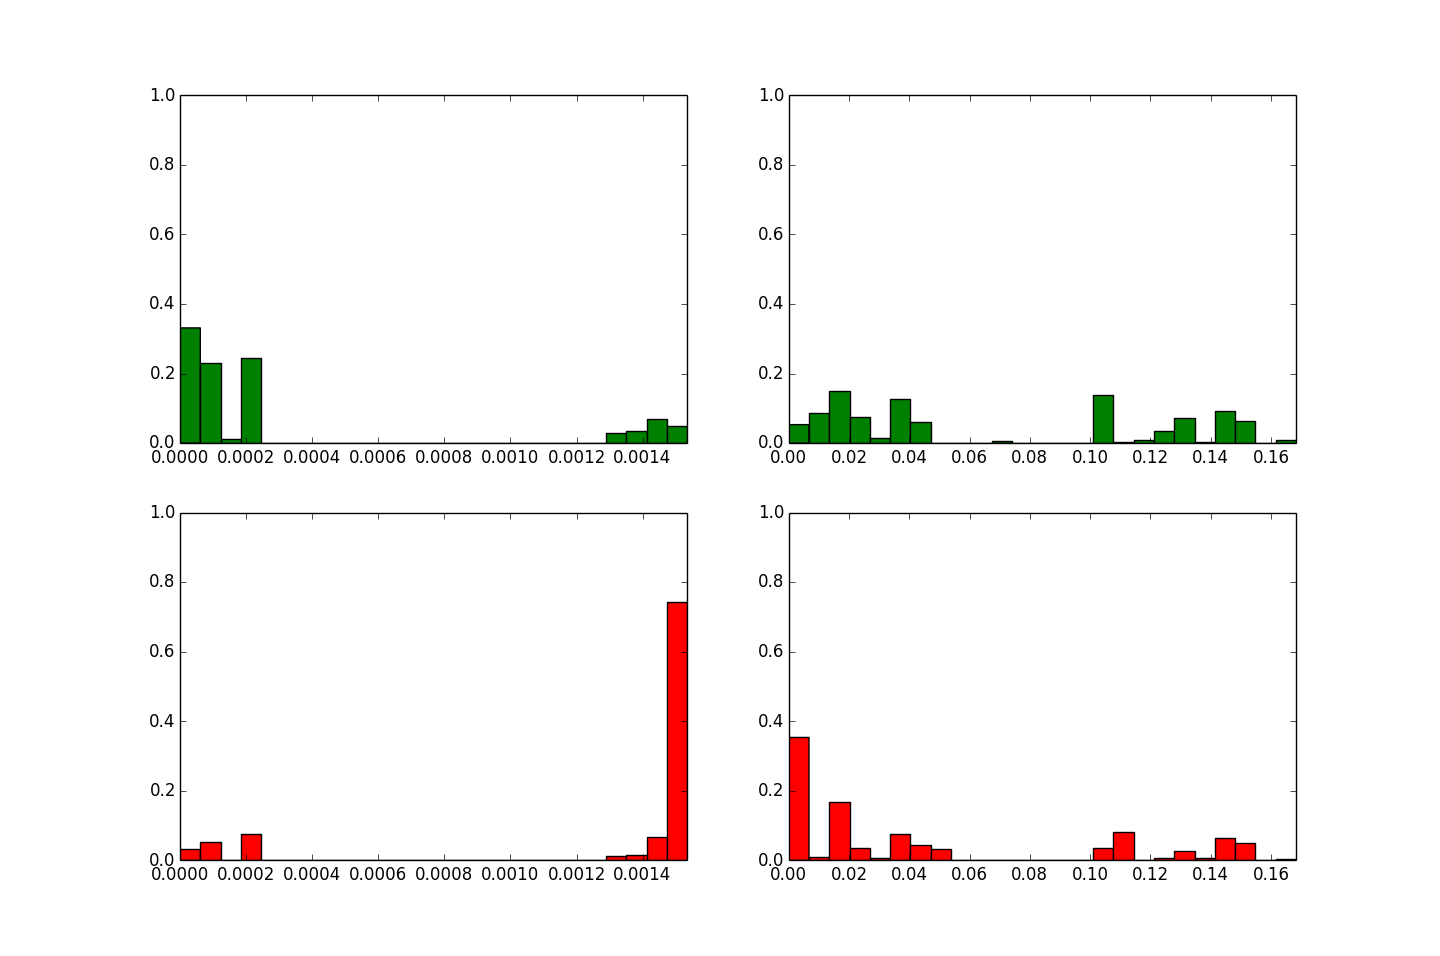
\includegraphics[width =\textwidth]{images/probabilities}
\caption{The distribution in percentages of correct (green) and incorrect (red) document links as proposed by a simple tag vectorizer that proposed all the documents in the dataset. Left hand side shows the tag probabilities and the right hand side the link probabilities. Thus, about 30\% of the correct links as proposed by the simple tag vectorizer have a probability between 0 and 0.00005.}
\label{distribution}
\end{figure}


\subsection{Threshold performance}
\begin{figure}[h!]
\begin{tabular}{cc}
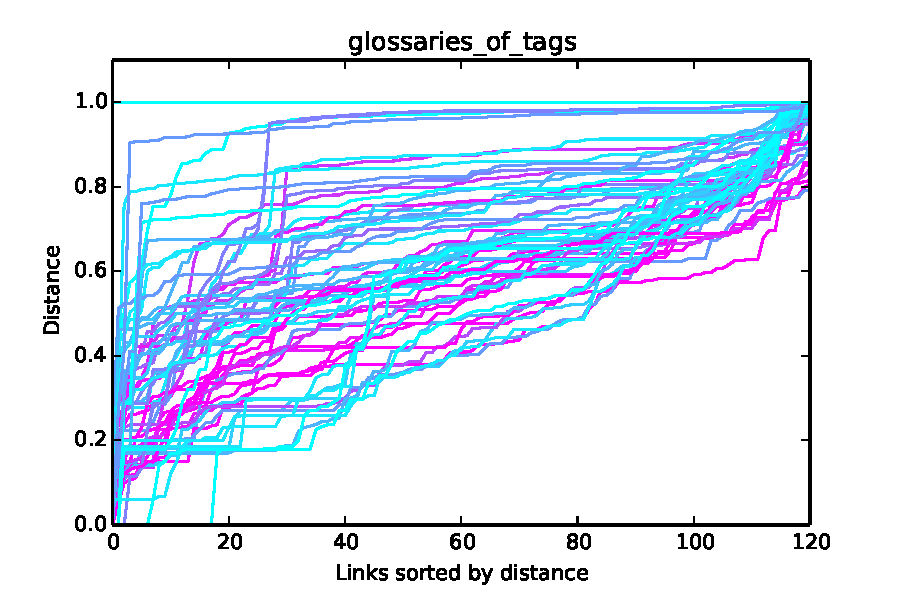
\includegraphics[width =0.5\textwidth]{images/thresh_cosine_glossaries_of_tags} 		& 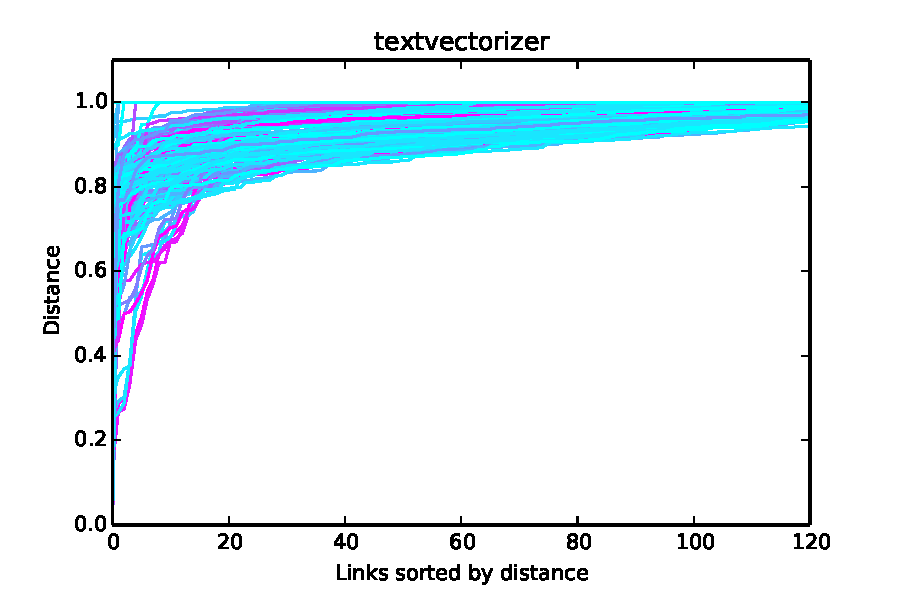
\includegraphics[width =0.5\textwidth]{images/thresh_cosine_textvectorizer} \\ \relax
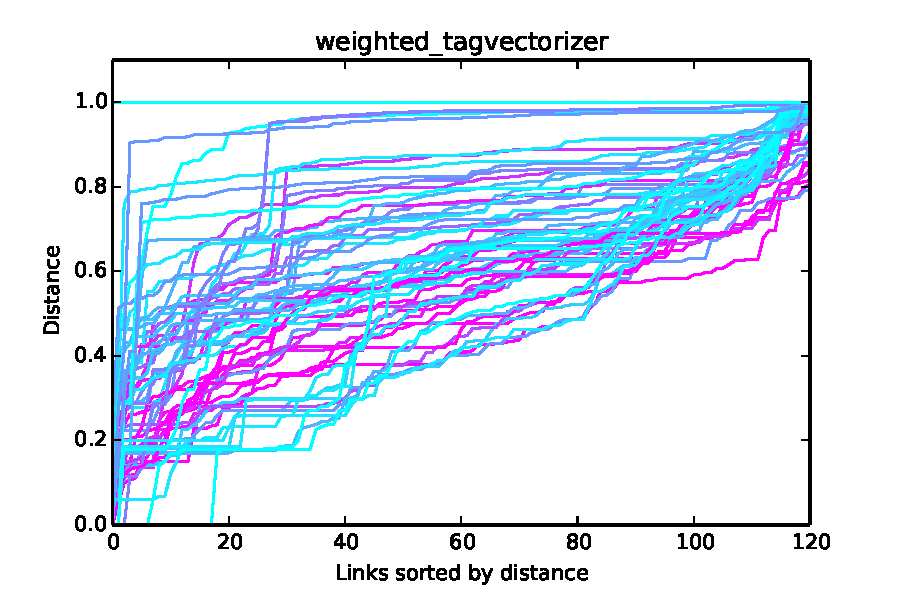
\includegraphics[width =0.5\textwidth]{images/thresh_cosine_weighted_tagvectorizer}	& 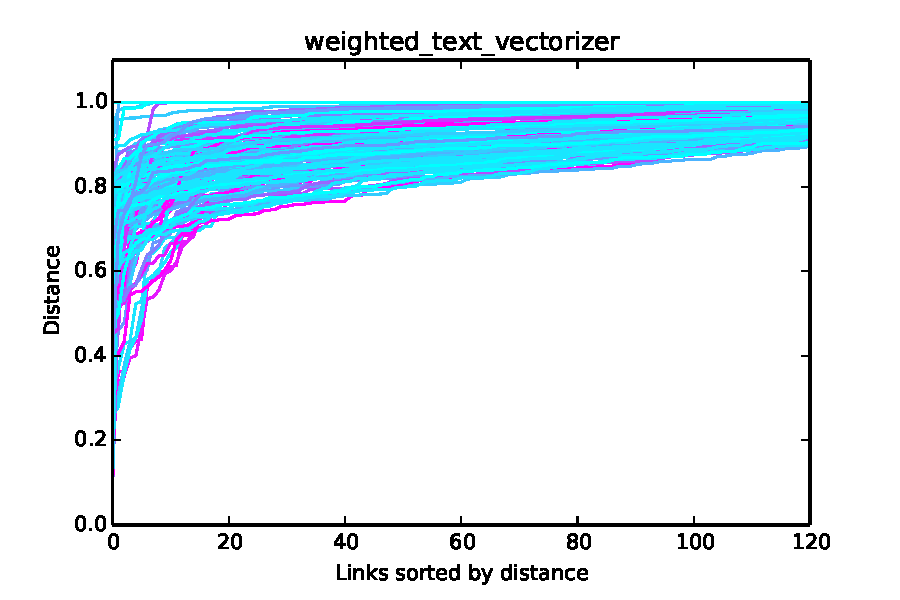
\includegraphics[width =0.5\textwidth]{images/thresh_cosine_weighted_text_vectorizer} \\ \relax
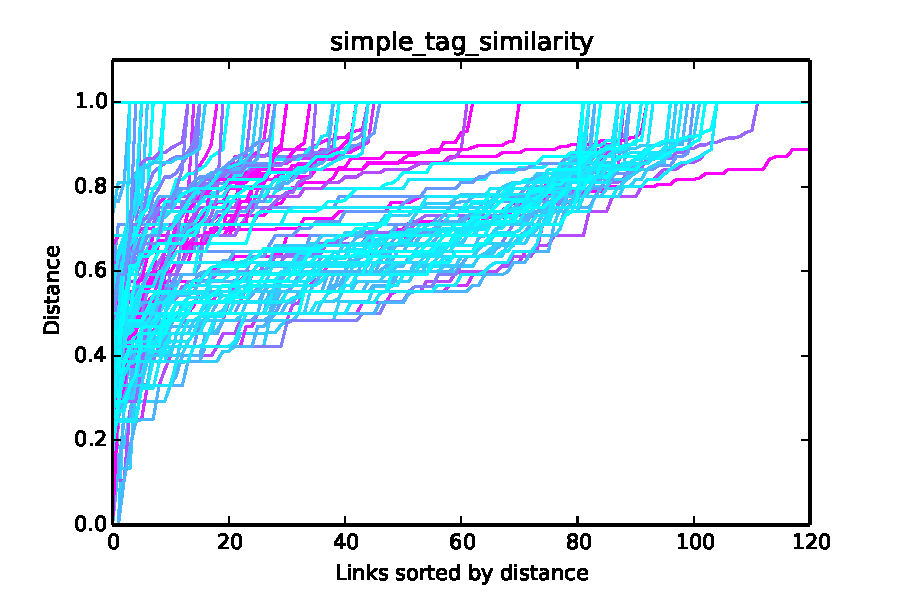
\includegraphics[width =0.5\textwidth]{images/thresh_cosine_simple_tag_similarity} 	& 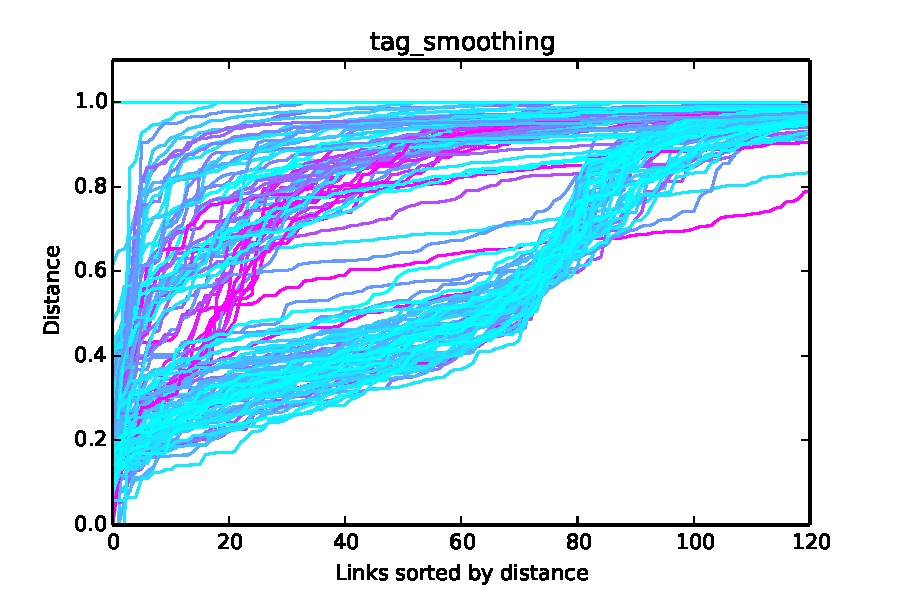
\includegraphics[width =0.5\textwidth]{images/thresh_cosine_tag_smoothing}
\end{tabular}
\caption{The sorted cosine distances of nearest neighbors and their distance for differend vectorizers. The blue purple gradient represents documents with 0 links (blue) to $\>10$ links (purple)}
\label{fig:thresholds}
\end{figure}

To evaluate the threshold, it is important to know what the result of the nearest neighbor 
algorithm is and how this relates to the way experts decide a document is relevant or 
not. Figure~\ref{fig:thresholds} shows the increase of distance for neighbors when ranked
less similar then their preceding neighbor.

Documents with little links registered in the original dataset are blueish in 
figure~\ref{fig:thresholds} and expected to have a small set of neighbors close 
by, after which the distance for the following neighbors should rise quickly. This 
general trend is visible in almost all tag vectorizers. 

Documents with more than average links registered in the original dataset are 
purplish in figure~\ref{fig:thresholds} and the neighbor distance is expected to increase
slower than the blue lines.

The results shown are very noisy, something that is to be expected from a small
human annotated dataset. However, we can detect anticipated general patterns.
Figure~\ref{fig:thresholds_differences} shows the differences between consecutive 
neighbors. In line with our understanding of expert linking, these graphs take the 
form of a long tail distribution for documents with a small amount of links.

\begin{figure}[h!]
\begin{tabular}{cc}
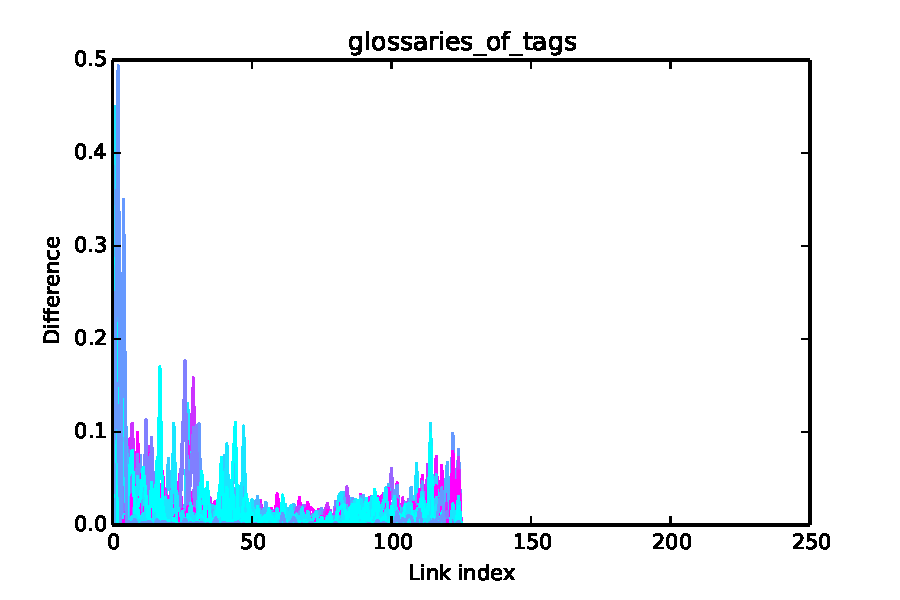
\includegraphics[width =0.5\textwidth]{images/thresh_cosine_glossaries_of_tags_distances} 		& 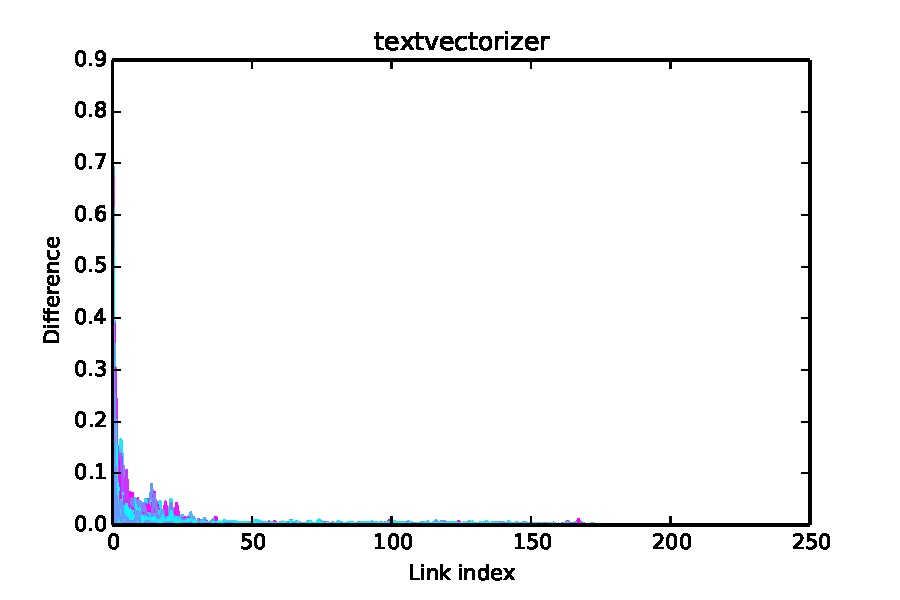
\includegraphics[width =0.5\textwidth]{images/thresh_cosine_textvectorizer_distances} \\ \relax
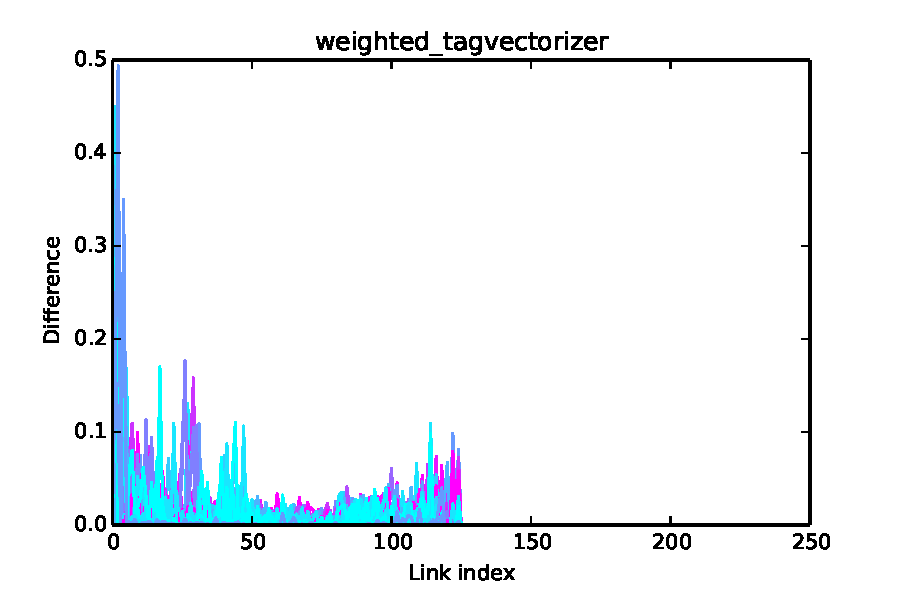
\includegraphics[width =0.5\textwidth]{images/thresh_cosine_weighted_tagvectorizer_distances}	& 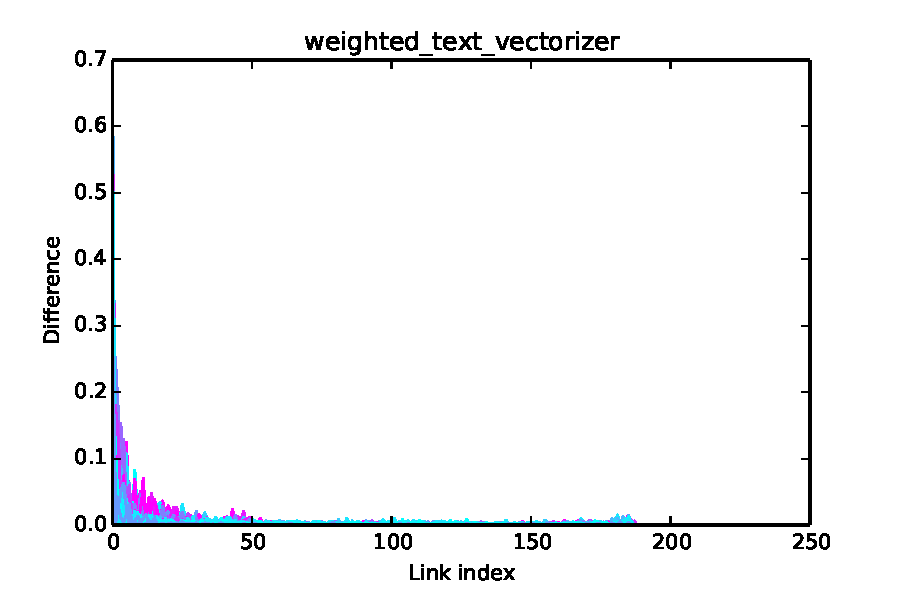
\includegraphics[width =0.5\textwidth]{images/thresh_cosine_weighted_text_vectorizer_distances} \\ \relax
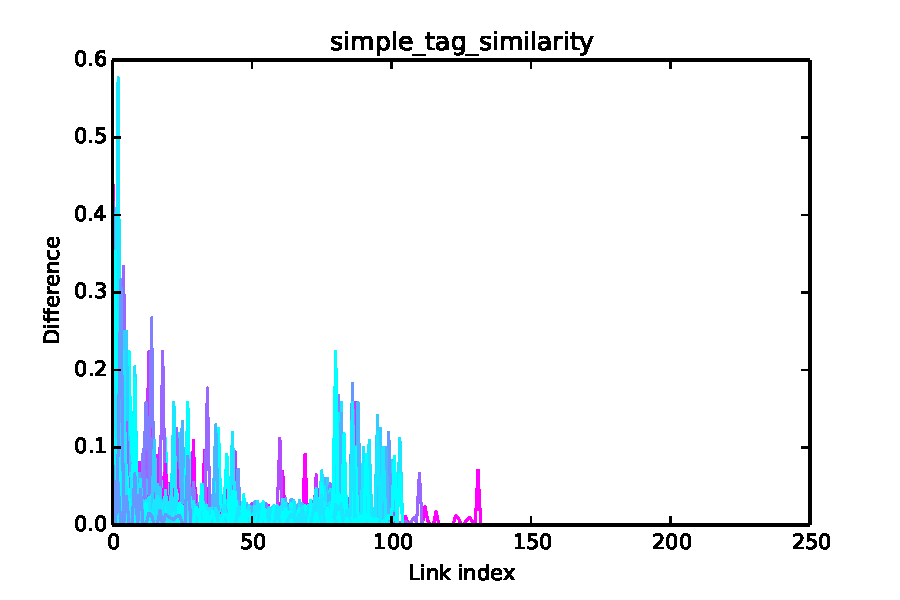
\includegraphics[width =0.5\textwidth]{images/thresh_cosine_simple_tag_similarity_distances} 	& 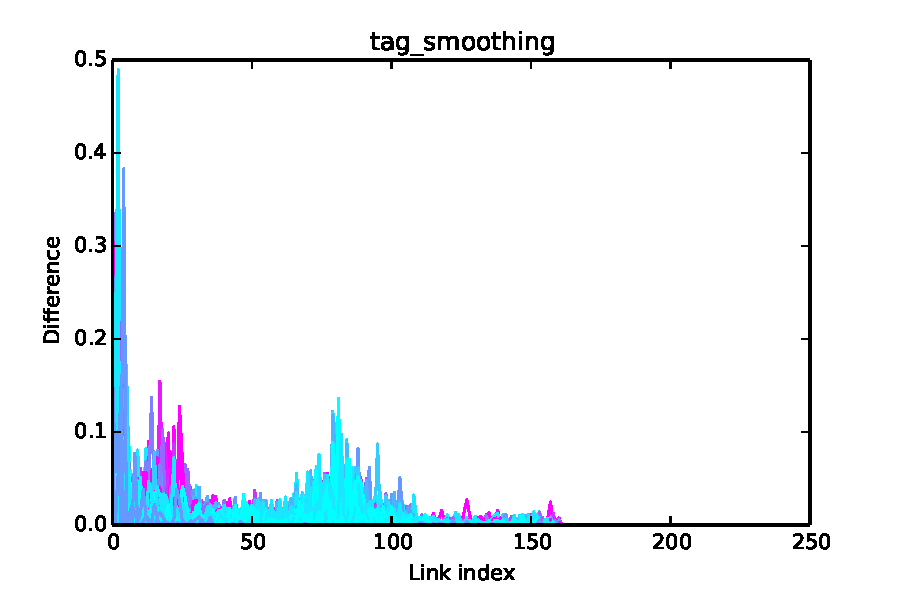
\includegraphics[width =0.5\textwidth]{images/thresh_cosine_tag_smoothing_distances}
\end{tabular}
\caption{Cosine distance differences betweeen two nearest neighbors sorted by document rank. The blue purple gradient represents documents with 0 links (blue) to $\>10$ links (purple)}
\label{fig:thresholds_differences}
\end{figure}

The above evidence suggests the nearest neighbor algorithm returns neighbours 
at distances in a similar to how experts would rate similarity. The reported decrease
of distance differences is expected and should be handled properly by the proposed
threshold calculation.

\begin{table}
\begin{tabular}{| l | l | l | l | l | l | l | l |}
\hline
THRESHOLD RECALL & Inf. &  Question &  Good Pr.& Project & Person &  Event & {\bf Average} \\
\hline
Textvectorizer & 12.05 & 39.65 & 19.64 & 20.73 & 5.21 & 21.43 & {\bf 15.66}\\
Weighted text & 14.80 & 29.82 & 19.64 & 24.37 & 5.24 & 21.43 & {\bf 15.11}\\
Simple tag & 24.14 & 20.61 & 48.21 & 30.63 & 19.49 & 26.19 & {\bf 23.26}\\
Tag smoothing & 26.20 & 21.93 & 55.35 & 23.85 & 22.05 & 46.83 & {\bf 25.42}\\
Glossaries of tags & 36.51 & 23.25 & 21.43 & 36.35 & 50.20 & 44.05 & {\bf 38.80}\\
Weighted tag & 36.52 & 23.25 & 21.43 & 36.35 & 50.20 & 44.05 & {\bf 38.80}\\
Hybrid & 24.14 & 41.40 & 48.21 & 30.63 & 20.34 & 26.19 & {\bf 27.26}\\
\hline

\hline
THRESH PRECISION & Inf. &  Question &  Good Pr.& Project & Person &  Event & {\bf Average} \\
\hline
Textvectorizer & 26.47 & 50.00 & 41.67 & 24.79 & 24.79 & 7.26 & {\bf 24.05}\\
Weighted text & 26.76 & 41.67 & 33.33 & 26.25 & 8.55 & 27.78 & {\bf 23.00}\\
Simple Tag & 28.43 & 17.54 & 62.60 & 56.25 & 10.77 & 38.89 & {\bf 23.71}\\
Tag smoothing &  23.77 & 17.11 & 50.00& 43.75 & 8.38 & 50.00 &{\bf 20.19 } \\
Glossaries of tags & 25.00 & 14.47 & 37.50 & 33.18 & 17.26 & 46.67 & {\bf 22.00}\\
Weighted tag & 25.00 & 14.47 & 37.50 & 33.18 & 17.26 & 46.67 & {\bf 22.00}\\
Hybrid & 28.43 & 39.91 & 62.50 & 56.25 & 13.33 & 38.89 & {\bf 28.61}\\
\hline
\\
\hline
THRESH F1-MEASURE & Inf. &  Question &  Good Pr.& Project & Person &  Event & {\bf Average} \\
\hline
Textvectorizer & 14.92 & 37.59 & 26.66 & 20.03 & 5.60 &  22.72 & {\bf 16.59 } \\
Weighted text & 16.53 & 31.47 & 23.06 & 23.24 & 6.58 & 23.33 & {\bf 16.57 } \\
Simple tag & 23.53 & 17.31 & 44.72 & 34.61 & 12.56 & 31.17& {\bf 20.27} \\
Tag smoothing & 22.04 & 17.54 & 45.23 & 29.76 & 11.26 & 48.29  &{\bf 19.49} \\
Glossaries of tags & 16.74 & 20.75 & 38.26 & 28.28 & 9.49 & 44.44 &{\bf 17.26} \\
Weighted tags & 16.74 & 20.75 & 38.26 & 28.28 & 9.49 & 44.44 &{\bf 17.26} \\
Hybrid &  23.53 & 35.31 & 44.72 & 34.61 & 13.85 & 31.17 &{\bf 23.92} \\
\hline
\end{tabular}

\caption{This table shows the precision, recall and F1 measure for all vectorizers per document type if they are thresholded with the parameter 0.3. All vectorizers used cosine distance. Thus, the first value 12.05 menas that the textvectorizer had a 12.5\% average precision documents of the type Information. }
\label{tab:thresh_eval}
\end{table}

Knowing that the pipeline until thresholding returns sane results, the actual performance
of the proposed threshold formula is tested on the dataset. The performance of the 
automated threshold was measured for all vectorizers with the cosine metric since that one gave the overall best reuslts. Now, precision and recall are different because the threshold can 
return a different number of links than the links that are known to be correct. Table~\ref{tab:thresh_eval} 
shows the precision, recall and f1-measure for each of the vectorizers, including an unraveling for
each type of document. A comparison between this table and table \ref{klink} and table \ref{hybrid}, which were measured with the k-link metric, shows that the f1-measure of most outcomes is comparable with the k-link accuracy that was measured, even though performance decreases a bit for all vectorizers. The hybrid vectorizer still performs the best. This difference in performance is probably due to the fact that k-link is optimistic with regards to both precision and recall, as explained in the evaluation metric of this chapter. % However, the glossaries of tags and weighted tag vectorizer seem to have significantly better results - an f1-measure of 28.08 compared to a 18.02 k-link measurement. This seems to be caused by a much higher precision and recall for the Person type of documents. In the knowledge base, a Person has on average about 1.6 links. However, the thresholded glossaries of tags returns 5.9 links on average. For example, the Person Andre Heck is linked to two documents, an Event and a Project. The k-link vectorizer returns two false documents - a Good Practice and a Qeustion. The thresholded vectorizer returns a total of 5 links, including the correct Event. It depends on a preference for recall or precision whether or not this difference in performance is desirable. 

\begin{table}

\end{table}
